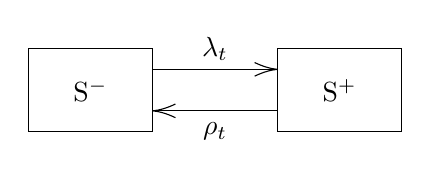
\begin{tikzpicture}[x=0.75pt,y=0.75pt,yscale=-1,xscale=1]
%uncomment if require: \path (0,300); %set diagram left start at 0, and has height of 300

\draw    (160, 120) rectangle (220, 160)   ;
\draw    (280, 120) rectangle (340, 160)   ;
\draw    (220,130) -- (280,130) ;
\draw [shift={(280,130)}, rotate = 180] [color={rgb, 255:red, 0; green, 0; blue, 0 }  ]   (0,0) .. controls (3.31,-0.3) and (6.95,-1.4) .. (10.93,-3.29)(0,0) .. controls (3.31,0.3) and (6.95,1.4) .. (10.93,3.29)   ;

\draw    (220,150) -- (280,150) ;

\draw [shift={(220,150)}, rotate = 0] [color={rgb, 255:red, 0; green, 0; blue, 0 }  ]   (0,0) .. controls (3.31,-0.3) and (6.95,-1.4) .. (10.93,-3.29)(0,0) .. controls (3.31,0.3) and (6.95,1.4) .. (10.93,3.29)   ;

\draw (190,140) node  [align=left] {S$^{-}$};
\draw (310,140) node  [align=left] {S$^{+}$};
\draw (250,120) node  [align=left] {$\lambda_t$};
\draw (250,160) node  [align=left] {$\rho_t$};
\end{tikzpicture}